\documentclass[a4paper,12pt,oneside,leqno]{scrartcl}%,12pt,oneside,reqno]{scrbook}
\usepackage{amsmath,amssymb,amsthm}
%\usepackage{listings}
%\usepackage{times}
\usepackage{lmodern}
\usepackage[T1]{fontenc}			% enable extra punctuation output 
\usepackage[english]{babel}		% the majority of this document is in German
\usepackage[pdftex]{hyperref}	% nice formatting for URLs 
\usepackage[top=2.5cm,bottom=2.5cm,left=3cm,right=3cm]{geometry}			% use the whole page
%\usepackage{setspace}			% allows us to double space 
\usepackage{color}
%\usepackage[none]{hyphenat}		% disables hyphenation
\usepackage[stable]{footmisc}	% allow footnote in section headings
\usepackage{natbib}				% extra bibliography tools
\usepackage{bibgerm}				% German APA like bibliography
%\usepackage{acronym}		
%\usepackage[parfill]{parskip}    % Activate to begin paragraphs with an empty line rather than an indent
%\usepackage{synttree}
\usepackage[pdftex]{graphicx}	% advanced graphics
%\usepackage{rotating}			% sidewaystable -- landscape'd table
%\usepackage{multirow}			% row-spanning cells in tables
%\usepackage{tabularx}			% a nifty expanded table environment
\usepackage{booktabs}			% professional looking tables
%\usepackage{longtable}
%\usepackage{lscape}
%\usepackage{epigraph}
\usepackage[utf8x]{inputenc}
\newcommand{\enquote}[1]{\frqq{}#1\flqq{}}
%\usepackage[utf8]{inputenc}
%\usepackage{csquotes}
%\usepackage{gb4e}  \noautomath	% necessary to make gb4e play nice
\usepackage{fixltx2e}
%\usepackage{paralist}
%\usepackage{tipa}
\usepackage{float}
%\usepackage{multicol}
%\begin{inparaenum}[\itshape a\upshape)] \item formatted within their paragraph; \item usually labelled with letters; and \item usually have the final item prefixed with ‘and’ or ‘or’,\end{inparaenum} like this example.
\usepackage{wrapfig}

% mark this is as a draft --- should work with all drivers
%\usepackage{draftwatermark}
%\SetWatermarkScale{.5}
%\SetWatermarkLightness{0.8}
%\SetWatermarkText{not for further distribution}

% Setup the PDF parts of the document
\hypersetup{
	 pdfauthor={Phillip M Alday},
	 pdftitle={Set Theory},
    bookmarks=true,
    bookmarksopen=true,
    pdfstartview=FitH
}

% natbib options
\bibpunct{(}{)}{;}{a}{~}{,}
\graphicspath{ {img/} }
%\newcommand{\HRule}{\rule{\linewidth}{0.5mm}}
\definecolor{darkgreen}{rgb}{0,0.6,0}

\theoremstyle{definition}
\newtheorem{defn}{Definition}

\newcommand{\fixme}[1]{\marginpar{\mbox{$<==$}}{\bfseries\color{blue}#1}}
\newcommand{\terminus}[1]{\textsc{#1}}
\newcommand{\bedeutung}[1]{`#1'}
\newcommand{\ortho}[1]{$\langle$#1$\rangle$}
\newcommand{\notation}[1]{\framebox[\textwidth]{\begin{minipage}[c]{0.99\textwidth}\textbf{Notation:} #1\end{minipage}}}
\newcommand{\application}[2]{\framebox[\textwidth]{\begin{minipage}[c]{0.9\textwidth}\textbf{Application: #1.} #2\end{minipage}}}

\newcommand{\super}[1]{^{#1}}

% this is basically a hack to fix bad hyphenation decisions from LaTeX :-(
%\hyphenation{Unter-stütz-ung}


\title{Set Theory}
\author{Phillip M Alday}
\date{Stand: 10. April 2012}

%\frenchspacing

\begin{document}
\newtheorem*{definition}{Definition}

\maketitle

\section{Basic Idea}
A \terminus{set} is a well-defined collection of objects, called \terminus{elements}.  The following are all sets:
\begin{gather} 
\left\{ \text{apple}, \text{grape}, \text{orange}, \text{banana} \right\} \\
\left\{ \checkmark{}, \maltese{}, \dag{}, \S,  \right\} \\
\left\{ w, x, y, z \right\}
\end{gather}

Sets can also be elements of another set --- it is possible to have a set of sets:
\begin{equation}
%\left\{ \left\{ \text{apple}, \text{pear}, \text{orange} \right\}, \left\{ \text{strawberry}, \text{raspberry}, \text{blueberry} \right\}, \left\{ \text{steak}, \text{sausage}, \text{hamburger} \right\}, \left\{ \text{zucchini}, \text{pumpkin}, \text{butternut} \right\} \right\}
\left\{ \left\{a,b,c \right\}, \left\{w,x,y,z\right\}, \left\{ \alpha, \beta \right\} \right\}
\end{equation}

\notation{Sets are represented by a capital letter: \[ A = \left\{ \alpha, \beta, \gamma, \delta\right\} \] }

Some sets are so important that they have a fixed symbol:
\begin{gather*}
\emptyset = \left\{ \right\} \\
\mathbb{N} = \left\{(0), 1, 2, 3, \ldots \right\} \\ % write this on the board using the definition
\mathbb{Z}= \left\{\ldots, -3, -2, -1, 0, 1, 2, 3, \ldots \right\} \\
\mathbb{Q} = \left\{\frac{p}{q} : p,q \in \mathbb{Z}, q \neq 0 \right\} \\
\end{gather*} 

%\subsection{Application: Types and Tokens}
%\application{Types and Tokens}{}

\section{Operations on Sets}
For the following, let $A,B, U$ be sets such that $A, B \subset U$.

\subsection{Equality of Sets}
Two sets $A, B$ are said to be \terminus{equal} if and only if they have the same elements. That is:
\begin{equation}
A = B \Longleftrightarrow \forall a \in A, a \in B \text{ and } \forall b \in B, b \in A
\end{equation}


\subsection{Sub- and Supersets}
A set $A$ is said to be a \terminus{subset} of a set $B$, if every element of $A$ is also in $B$: 
\begin{equation}
A \subset B \Longleftrightarrow \forall a \in A, a \in B
\end{equation}
Correspondingly, $B$ is said to be a \terminus{superset} of $A$.

Please note that a set is a subset of itself and a superset of itself according to these definitions.  If we do not wish to include the original set itself when discussing subsets and supersets, we use the modifier \terminus{proper}.

\notation{We can also indicate that only proper sub- or supersets are allowed:
\begin{equation}
A \subsetneq B
\end{equation}
Likewise, we can emphasize that non proper sub- or supersets are allowed:
\begin{equation}
A \subseteq B
\end{equation}
}

\subsection{Complement}
\begin{wrapfigure}{r}{3cm}
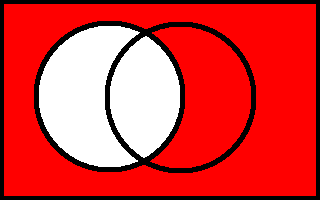
\includegraphics[height=2cm]{set-base-lettered-complement-left}
\vspace{-20pt}
\caption{Set~Complement.}\label{fig:sets-complement}
\vspace{-20pt}
\end{wrapfigure}
The \terminus{complement} of $A$ in $U$ is the set of elements in $U$ but not in  $A$. That is:
\begin{equation}
A^{c} = \left\{ x \in U : x \not\in A \right\}
\end{equation}
Please note: set complement requires the context of another set!

\subsection{Intersection}
\begin{wrapfigure}{r}{3cm}
%\begin{figure}
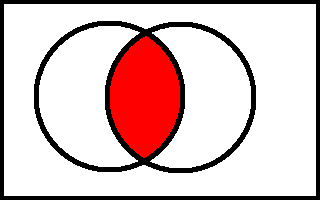
\includegraphics[height=2cm]{set-base-lettered-intersection}
\vspace{-20pt}
\caption{Intersection.}\label{fig:sets-intersection}
\vspace{-20pt}
\end{wrapfigure}
The \terminus{intersection} of $A$ and $B$ is the set of elements in both $A$ and $B$. That is:
\begin{equation}
A \cap B = \left\{x: x \in A \text{ and } x \in B \right\}
\end{equation}
This is, roughly, the overlap between the two sets.

\subsection{Union}
\begin{wrapfigure}{r}{3cm}
%\begin{figure}
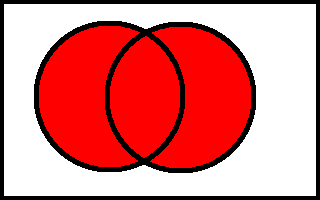
\includegraphics[height=2cm]{set-base-lettered-union}
\vspace{-20pt}
\caption{Union.}\label{fig:sets-union}
\vspace{-20pt}
\end{wrapfigure}
The \terminus{union} of $A$ and $B$ is the set such that each element is in $A$ or is in $B$ (or both):  
\begin{equation}\label{eq:uniondef}
A \cup B = \left\{x: x \in A \text{ or } x \in B \right\}
\end{equation}
This is roughly the set you get from combining $A$ and $B$.  Please note: this does not double any elements already found in both sets (the intersection); if any doubt, use the formal definition (\ref{eq:uniondef})!
\pagebreak

\subsection{Difference (Relative Complement)}
\begin{wrapfigure}{r}{3cm}
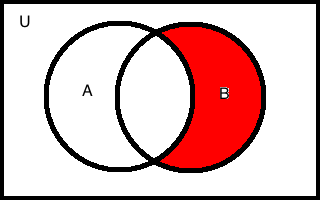
\includegraphics[height=2cm]{set-base-lettered-difference}
\vspace{-20pt}
\caption{Difference}\label{fig:sets-difference}
\vspace{-20pt}
\end{wrapfigure}
The \terminus{difference} of $B$ and $A$ is the set of elements in $B$ but not in $A$:  
\begin{equation}
B \setminus A = \left\{ x \in B, x \not\in A\right\}
\end{equation}
This is roughly the set you get from cutting out  $A$ from $B$. The $\setminus$~symbol even looks a little bit like a cutting implement \ldots

\subsection{Disjoint Union}
\begin{wrapfigure}{r}{3cm}
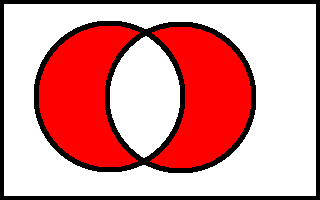
\includegraphics[height=2cm]{set-base-lettered-symmetricdifference}
\vspace{-20pt}
\caption{Disjoint Union}\label{fig:sets-disjointunion}
\vspace{-20pt}
\end{wrapfigure}
The \terminus{disjoint union} of $A$ and $B$ is the set of elements either in $A$ or in $B$, but not both: 
\begin{equation}
A \sqcup B = \left\{x: x\in A \text{ xor } x \in B\right\}% = \left(A\cup{}B\right) \setminus \left(A\cap{}B\right)  
\end{equation}
This is roughly the parts of $A$ and $B$ which don't have any overlap.

\section{Size (Cardinality)}
%The size or \terminus{cardinality} of a set is also an important notion. It provides us with a way to compare sets and provides
The \terminus{cardinality} of a set corresponds to the intuitive notion of \enquote{size}: the number of elements in a set.  For example,
\begin{gather}
\left| \emptyset \right| =  0 \\
\left| \left\{ 1 \right\} \right| = 1 \\
\left| \left\{ 1, 2 \right\} \right| =  2 \\
\left| \left\{ \checkmark{}, \maltese{}, \dag{}, \S,  \right\} \right| =  4 \\
\left| \left\{ 1, 2, \ldots, 100 \right\} \right| =  100 \\
\left| \left\{ 1, 2, \ldots, n \right\} \right| = n\label{eq:card-n}  \\
\left| \mathbb{N} \right| = ?    
\end{gather}
As we can see, this is pretty easy for finite sets, even arbitrarily large ones.\footnote{It is very important to realize that \enquote{arbitrarily large} is not the same as \enquote{infinite}.  Equation (\ref{eq:card-n}) shows this: this works for any natural number (of which there are infinitely many), but does not work for the truly infinite case.} But what happens if we want to measure the size of infinite sets?  As it turns out, there are different infinities.  Broadly speaking, there are two major types of infinity. \terminus{Countably infinite} sets can be enumerated or counted in the same way as the natural numbers: if we had infinitely much time, we could count them off one by one, in much the same way as we can start counting from one and keep going forever.\footnote{Formally, an infinite set $X$ has countably many elements if there exists a bijection (a one-to-one and onto function) between $X$ and $\mathbb{N}$}.  The integers ($\mathbb{Z}$) are also countable, we count them off like so: $0, 1, -1, 2, -2, 3, -3, \ldots$.\footnote{Challenge question: What would this bijection look like formally?}

In contrast to the integers, we can't count off the reals ($\mathbb{R}$). If we start with 1, we can't say what comes next: 1.1? 1.01? 1.001? 1.0001?  We can always add another zero: the reals are a continuum. This type of infinity is somehow different and intuitively \enquote{bigger}.  Indeed, the countable subsets of the reals are all proper subsets, and so we can somehow say that uncountable infinity is somehow \enquote{bigger} than the countable ones.

But here is also a good time to note that things are a little bit weird when dealing with infinity.  The natural numbers are a proper subset of the integers, yet they are both countably infinite, which means they both have the same size in some sense. Similar things can happen with uncountable infinities: the closed interval $\left[0,1\right]$ can be used to represent all real numbers without \enquote{losing} any.\footnote{The easiest example of how a finite interval can be mapped onto the entire real line is provided by high school trigonometry.  The tangent function provides a bijection between the open interval $(-\pi,\pi)$ and $(-\infty, \infty)$, so the two sets are also somehow the same \enquote{size}.} This fact is frequently used in optimality theory and computational linguistics as well as probability and statistics.  A weight or a probability or any other type of scaling factor is typically represented as a number between 0 and 1, inclusive.  Resolving this weirdness is well beyond the scope of this introduction, but the lesson here is simple: be wary of doing \enquote{normal} things around infinity or treating it like a number, because it's not.

\section{Exercises}
\begin{enumerate}
\item Restate the disjoint union operation in terms of intersections and unions.
\item Give a formula for $|A \cup{} B|$ in terms of $A,B$ and other basic operations on them. 
\item Is the union of two countable sets also countable?
\item What are the cardinalities of the following sets?
	\begin{enumerate}
	\item \{ the numbers between 218 and 527, inclusive \}
	\item \{ distinct rearrangements of the letters in \enquote{Dana} \}
	\end{enumerate}
\end{enumerate}

\phantomsection	% this fixes some pagination/link issues with the bibliography
%\cite{*}
\bibliographystyle{gerapali}
%\addcontentsline{toc}{chapter}{Literaturverzeichnis}
%\bibliography{alday}
\end{document}